\documentclass[xcolor=table]{beamer}

\uselanguage{English}
\languagepath{English}
\usetheme{HongKong}
\useinnertheme{rounded}
\usepackage{color, colortbl}
\usepackage{tcolorbox}
\usepackage{multirow} 
\usepackage{textcomp}
\usepackage{siunitx}
\usepackage{tikz}
\usepackage[utf8]{inputenc}
\usepackage[safe]{tipa}
\usepackage{array}
\usepackage{hhline}
\usepackage{pbox}

\usepackage{etoolbox}

\usepackage{algorithm,algorithmic}
%\usepackage[noend]{algpseudocode}

\tikzset{rndblock/.style={rounded corners,rectangle,draw,outer sep=0pt}}
\newcommand{\tframed}[2][]{\tikz[baseline=0.1pt]\vspace{0.1cm}\node[rndblock,minimum height=1.5em,#1] (m) {#2} ;}
\newcommand{\hilight}[1]{\textbf{\tframed[blue,fill=blue!10]{#1}}}
\newcommand{\whilight}[1]{\textbf{\tframed[purple,fill=purple!10]{#1}}}

\newcommand{\sP}{\hspace{1pt}}
\newcommand{\mP}{\hspace{3pt}}
\newcommand{\bP}{\hspace{6pt}}
\newcommand{\BP}{\hspace{12pt}}


\newcolumntype{L}[1]{>{\raggedleft\let\newline\\\arraybackslash\hspace{0pt}}m{#1}}

%\newcommand{\hilight}[1]{\colorbox{white}{#1}}

%==============================================================================================================

\setbeamertemplate{navigation symbols}{}
\setbeamertemplate{items}[ball] 
\setbeamertemplate{blocks}[rounded][shadow=true,width=.7\textwidth] 

\setbeamercolor{myBlueBox} {bg=blendedblue, fg=white}
\setbeamercolor{myGrayBox} {bg=blendedgray, fg=black}

\definecolor{darksalmon}{RGB}{233,150,122}
\definecolor{blendedblue}{rgb}{0.137,0.466,0.741}
\definecolor{blendedgray}{rgb}{0.838,0.833,0.833}
\definecolor{blendedpurple}{RGB}{75,20,130}
\definecolor{tgray}{rgb}{0.211, 0.211,0.244}
\definecolor{darkgray}{rgb}{0.450,0.450,0.450}
\definecolor{maroon}{rgb}{0.665, 0.142, 0.142}
\definecolor{ngreen}{rgb}{0.000,0.500,0.000}

\newcolumntype{g}{>{\columncolor{tgray}}S[tabformat=2.2]}

\newenvironment<>{varblock}[2][\textwidth]{%
\vspace*{-20pt}
	  \setlength{\textwidth}{#1}
	  \begin{actionenv}#3%
	    \def\insertblocktitle{#2}%
	    \par%
	    \usebeamertemplate{block begin}}
	  {\par%
	    \usebeamertemplate{block end}%
	  \end{actionenv}
\vspace*{-20pt}
}


%\setbeamertemplate{itemize item}{$\blacktriangleright$}
\setbeamertemplate{itemize subitem}{$\ast$}
\setbeamerfont{itemize/enumerate subbody}{size=\footnotesize} 							%to set the body size
%\setbeamertemplate{itemize subitem}{\tiny\raise1.25pt\hbox{\donotcoloroutermaths$\blacktriangleright$}}  	%to set the symbol size


%==============================================================================================================

\title{Detection of sentence modality on French automatic speech-to-text transcriptions}
\author[Luiza Orosanu, Denis Jouvet]
{
\vskip0.3cm \textbf{Luiza Orosanu, Denis Jouvet}
\vskip0.45cm  INRIA-Loria, Nancy, France  \\
\vskip0.15cm Multispeech Team\vspace{-1cm}
}
\date{}

\AtBeginSection[]
{
  \begin{frame}
	\thispagestyle{empty}
   	\frametitle{Summary}
	\tableofcontents[currentsection, hideothersubsections,sectionstyle=show/shaded, subsectionstyle=show/shaded/hide] 	%subsectionstyle=show/shaded,currentsection,subsections, currentsubsection]
  \end{frame}
}


\AtBeginSubsection[]
{
  \begin{frame}
	\thispagestyle{empty}
   	\frametitle{Summary}
	\tableofcontents[currentsubsection, hideothersubsections,sectionstyle=show/shaded, subsectionstyle=show/shaded/hide] 	
  \end{frame}
}


\newcommand{\firstslide}{%
	\begin{frame}
	\hfill
	\thispagestyle{empty}
	\titlepage
	\end{frame}
}

%==============================================================================================================
\begin{document}
\renewcommand{\inserttotalframenumber}{19}

%==============================================================================================================
\firstslide


%==============================================================================================================
\section{Context}
\begin{frame}[t]{Context}
\setcounter{framenumber}{1}

{\scriptsize \textbf{\color{purple}Objective} : state from the automatic transcription if the sentence \\\hskip12ex is a question or a statement }
%inform the deaf people if a question was directed to them

\bigskip
\begin{center}
\vskip-3ex
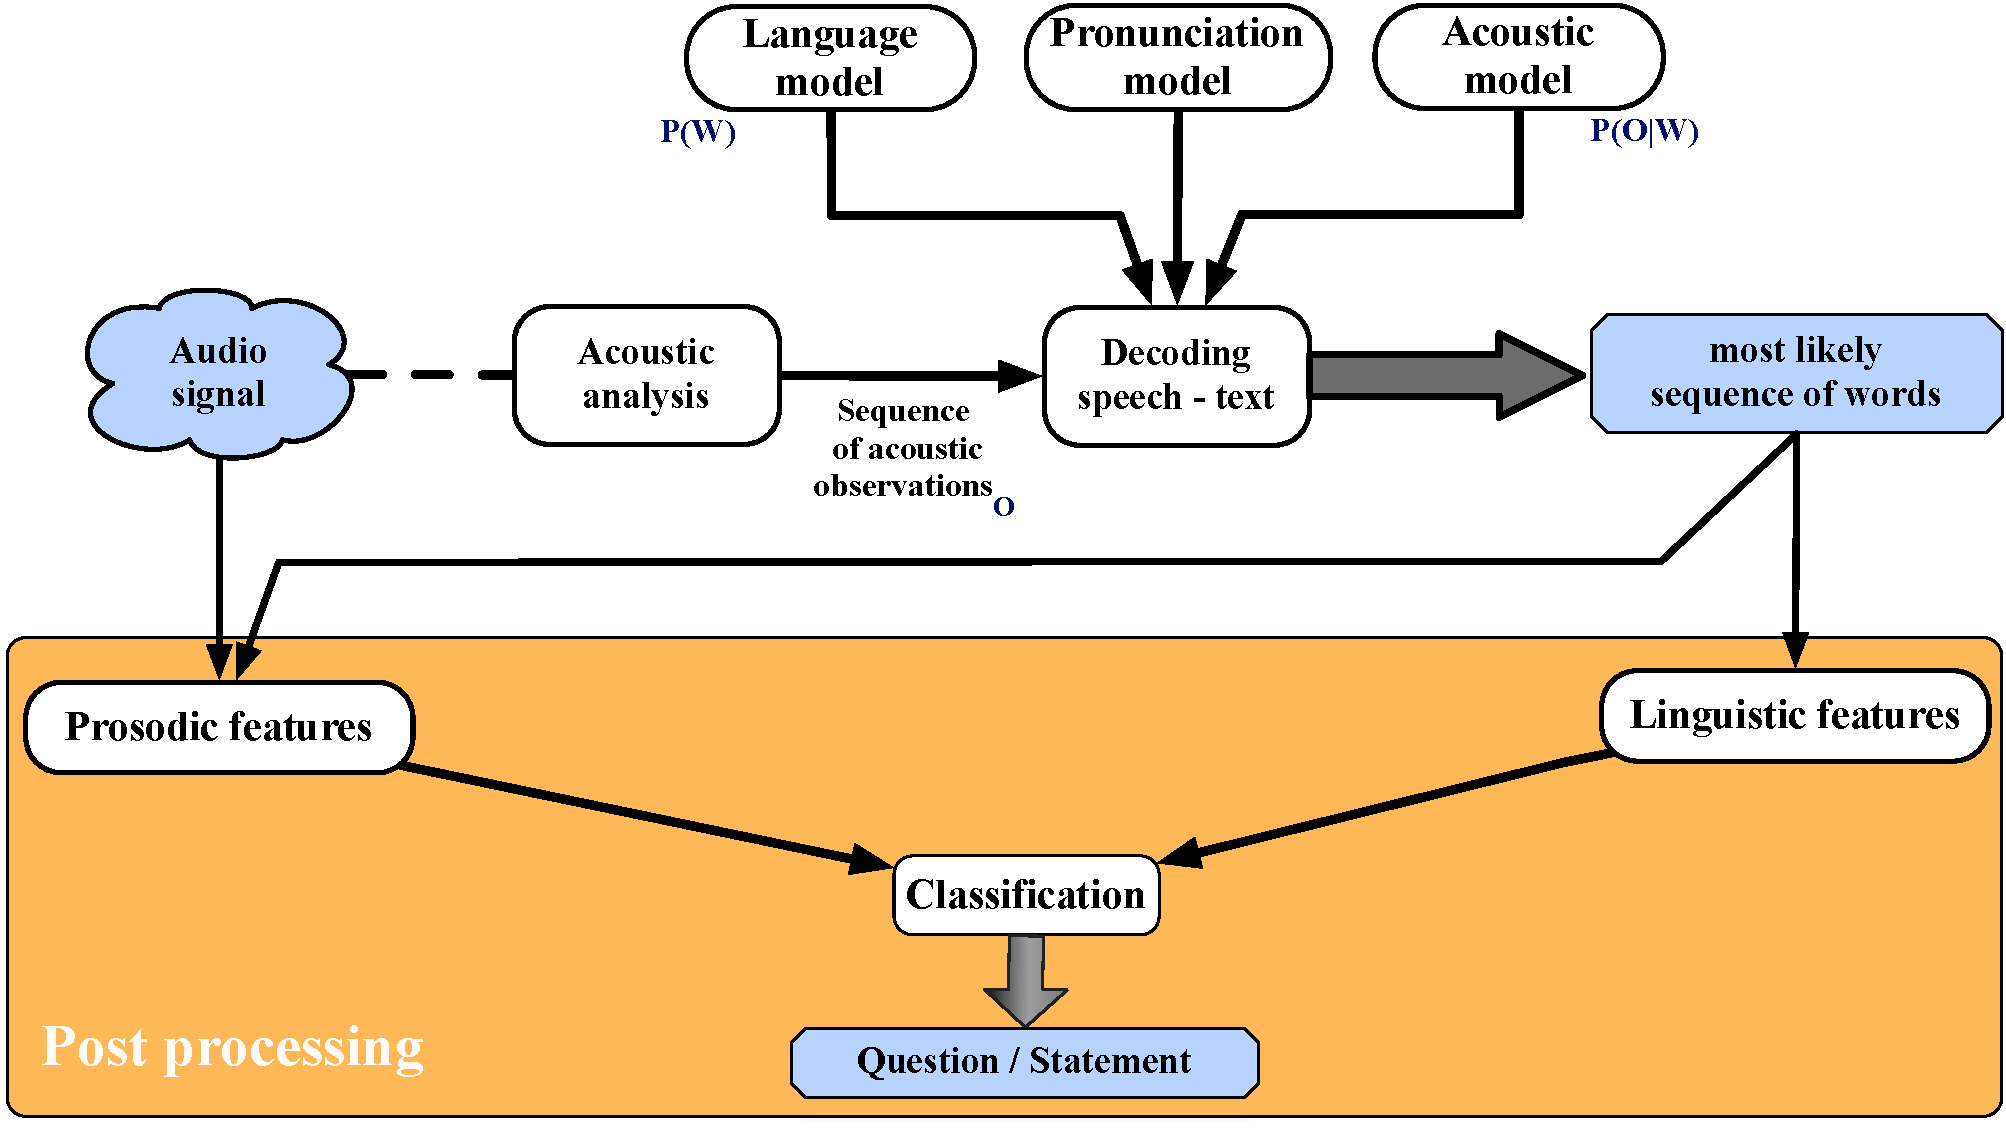
\includegraphics[scale=0.32]{Image/picture/QD_last_en.pdf}
\end{center}


\end{frame}


%==============================================================================================================
\begin{frame}[t]{Context}

\vskip0.3cm
Two types of questions

\begin{itemize}
\vskip3ex 
\item expressed with interrogative forms 
	\begin{itemize}
	\smallskip
	\item qu'est ce qu'on doit comprendre ?
	\smallskip
	\item est ce que vous souhaitez une confrontation ?
	\smallskip
	\item quelles sont les grandes annonces hein à attendre ?
	\end{itemize}
		
	
\vskip3ex
\item perceived as questions only through the intonation

	\begin{center}
	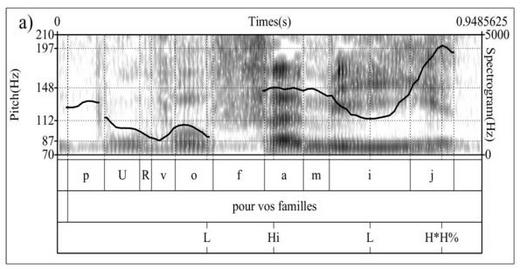
\includegraphics[scale=0.45]{Image/picture/prosodie}
	\end{center}
	
\end{itemize}

\end{frame}

%==============================================================================================================
\begin{frame}[t]{Context}

\begin{itemize}

\vskip1.5cm
\item study several approaches
	\begin{itemize}
	\bigskip
	\item prosodic classifier: uses intonation
	\bigskip
	\item linguistic classifier: uses the linguistic information
	\bigskip
	\item combined classifier: uses both types of information
	\end{itemize}
	
\end{itemize}
\end{frame}


%==============================================================================================================
\section{Approach}
\begin{frame}[t]{Prosodic features (\#10)}
\setcounter{framenumber}{4}

\vskip1.2cm
\begin{itemize}

\item generally, a question has a final rising pitch
	
\bigskip
\item we compute 10 prosodic features that take into account 

\vskip1ex
	\begin{columns}
	\begin{column}{.35\textwidth}
	   	\begin{list}{$\ast$}{\leftmargin=17mm \itemindent=0em}
	 	\item \footnotesize{the duration}
	 	\item \footnotesize{the energy}
	 	\item \footnotesize{the pitch}
	 	\end{list}
	\end{column}
	{\vrule height 0.8cm width 0.4pt} 
	\begin{column}{.65\textwidth}
	 	\hskip0.3cm \footnotesize{of the last prosodic group of the sentence}
	\end{column}
	\end{columns}

\end{itemize}

\end{frame}



%==============================================================================================================
\begin{frame}[t]{Prosodic features (\#10)}

\vskip0.3cm
\textbf{\color{purple}Features vector}

{
\bigskip
\scriptsize
\renewcommand{\arraystretch}{1.3}
\begin{tabular}{|c|p{2.5cm}cp{6.5cm}|}
\hline
{\scriptsize \textbf{class}} 	& \multicolumn{3}{l|}{\{0=statement; 1=question\}}						\\ \hline
\parbox[t]{2mm}{\multirow{10}{*}{\rotatebox[origin=c]{90}{\scriptsize \textbf{Prosodic Features}}}}
	& {VNDurNorm}		& = & \hskip-2ex the duration of the last syllable (normalized)					\\ \cline{2-4}
	& {VNLogENorm}		& = & \hskip-2ex the logarithm of the energy of the last syllable (normalized)			\\ \cline{2-4}
	& {VNF0Delta}		& = & \hskip-2ex the F0 difference between the last syllable and the first syllable		\\ \cline{2-4}
	& {VNF0Slope}		& = & \hskip-2ex the F0 slope on the last syllable						\\ \cline{2-4}
	& {VNF0SlopeT2}		& = & \hskip-2ex VNF0Slope * VNDurNorm$^2$							\\ \cline{2-4}
	& {globalSlopeSlope}	& = & \hskip-2ex the F0 slope on the longest ending F0 slope					\\ \cline{2-4}
	& {globalSlopeLength}	& = & \hskip-2ex the length of the longest ending F0 slope					\\ \cline{2-4}
	& {globalSlopeDelta}	& = & \hskip-2ex the F0 difference between the beginning and the end of the longest ending F0 slope \\ \cline{2-4}
	& {globalSlopeSlopeT2}	& = & \hskip-2ex globalSlopeSlope * globalSlopeLength$^2$					 \\ \cline{2-4}
	& {lastF0Level}		& = & \hskip-2ex the last F0 level (normalized by speaker)					\\ \hline
         		
\end{tabular}
}

\end{frame}

%=============================================================================
\begin{frame}[t]{Linguistic features (\#3)}

\vskip0.4cm
\begin{itemize}
\item \textbf{\color{blendedblue} iP}: the interrogative patterns
	\vskip2ex\hskip6ex $\rightarrow$ indicate the presence or absence \\\hskip6ex of an interrogative pattern in a phrase
\end{itemize}

\vskip2ex
\begin{columns}
	\begin{column}{.22\textwidth}
	\begin{itemize}
	\item[\color{blendedblue}$\ast$] quel
	\item[\color{blendedblue}$\ast$] quelle
	\item[\color{blendedblue}$\ast$] quels
	\item[\color{blendedblue}$\ast$] quellles
	\item[\color{blendedblue}$\ast$] comment
	\item[\color{blendedblue}$\ast$] combien
	\end{itemize}
	\end{column}
	\begin{column}{.3\textwidth}
	\begin{itemize}
	\item[\color{blendedblue}$\ast$] pourquoi
	\item[\color{blendedblue}$\ast$] est ce que
	\item[\color{blendedblue}$\ast$] est ce qu'
	\item[\color{blendedblue}$\ast$] qu' est ce
	\item[\color{blendedblue}$\ast$] qu' est ce que
	\item[\color{blendedblue}$\ast$] qu' est ce qu'
	\end{itemize}
	\end{column}
	\begin{column}{.01\textwidth}
	\end{column}
\end{columns}



\end{frame}


%=============================================================================
\begin{frame}[t]{Linguistic features (\#3)}

\vskip3ex

\begin{itemize}
\item the probability of the sentence being a question 
	
	\begin{itemize}
	\vskip2ex
	\item with respect to two reference language models
	\end{itemize}
	
	\vskip1.1ex
	\footnotesize 
	\begin{columns}
	\begin{column}{.1\textwidth}
	\end{column}
	\begin{column}{.67\textwidth}
	   	$$\text{LLR(sentence)}=\text{Log}\left(\frac{\text{P(sentence} \rvert \text{\color{purple}LM-question)}}{\text{P(sentence} \rvert \text{\color{purple}LM-statement)}}\right)$$

	   	\vskip1ex
		$\ast$ LLR $\geq$ 0  $\rightarrow$ likely to be a question \\
		$\ast$ LLR $\textless$ 0 $\rightarrow$ likely to be a statement
	\end{column}
	\begin{column}{.09\textwidth}
	\end{column}
	\begin{column}{.37\textwidth}
		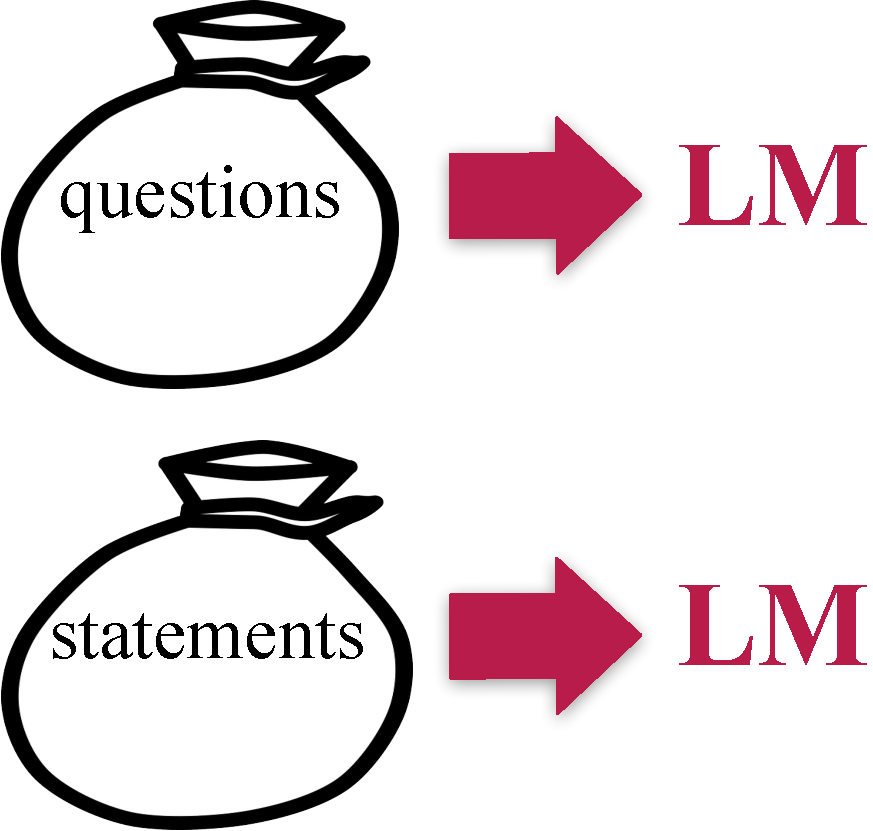
\includegraphics[scale=0.19]{Image/picture/LM-qs.pdf}
	\end{column}
	\end{columns}
\end{itemize}

\vskip5ex
\begin{center}	
	\vskip-1.3ex
	\begin{beamerboxesrounded}[width=0.85\textwidth,shadow=false]{}
	{\scriptsize

	\begin{tabular}{p{1cm}|p{7cm}}
	\multirow{2}{*}{\textbf{lexLLR}}	& we apply the \textbf{\color{purple}lexical} language models 	\\ 
						& on the \textbf{\color{purple}sequence of words}			\\
	\end{tabular}
	}
	\end{beamerboxesrounded}
\end{center}

\smallskip
\begin{center}
	\vskip-5ex
	\begin{beamerboxesrounded}[width=0.85\textwidth,shadow=false]{}
	{\scriptsize
	\begin{tabular}{p{1cm}|p{7cm}}
	 \multirow{2}{*}{\textbf{synLLR}} 	& we apply the \textbf{\color{purple}syntactic} language models	\\ 		
						& on the \textbf{\color{purple}sequence of POS tags}			\\ 
	\end{tabular}
	}
	\end{beamerboxesrounded}
\end{center}

\end{frame}

%==============================================================================================================
\begin{frame}[t]{Combined linguistic-prosodic features (3L-10P)}

\vskip-1ex
\textbf{\color{purple}Features vector}

{
\bigskip
\scriptsize
\renewcommand{\arraystretch}{1.3}
\begin{tabular}{|c|p{2.5cm}cp{6.5cm}|}
\hline
{\scriptsize \textbf{class}} 	& \multicolumn{3}{l|}{\{0=statement; 1=question\}}						\\ \hline\hline	
\parbox[t]{2mm}{\multirow{3}{*}{\rotatebox[origin=c]{90}{\scriptsize \textbf{3L}}}}
	& {lexLLR}		& = & \hskip-2ex {\scriptsize the lexical log-likelihood ratio}					\\ \cline{2-4}
	& {synLLR}		& = & \hskip-2ex {\scriptsize  the syntactic log-likelihood ratio}				\\ \cline{2-4}
	& {iP}			& = & \hskip-2ex {\scriptsize  presence or absence of interrogative pattern}			\\ \hline\hline	
\parbox[t]{2mm}{\multirow{10}{*}{\rotatebox[origin=c]{90}{\scriptsize \textbf{10P}}}}
	& {VNDurNorm}		& = & \hskip-2ex the duration of the last syllable (normalized)					\\ \cline{2-4}
	& {VNLogENorm}		& = & \hskip-2ex the logarithm of the energy of the last syllable (normalized)			\\ \cline{2-4}
	& {VNF0Delta}		& = & \hskip-2ex the F0 difference between the last syllable and the first syllable		\\ \cline{2-4}
	& {VNF0Slope}		& = & \hskip-2ex the F0 slope on the last syllable						\\ \cline{2-4}
	& {VNF0SlopeT2}		& = & \hskip-2ex VNF0Slope * VNDurNorm$^2$							\\ \cline{2-4}
	& {globalSlopeSlope}	& = & \hskip-2ex the F0 slope on the longest ending F0 slope					\\ \cline{2-4}
	& {globalSlopeLength}	& = & \hskip-2ex the length of the longest ending F0 slope					\\ \cline{2-4}
	& {globalSlopeDelta}	& = & \hskip-2ex the F0 difference between the beginning and the end of the longest ending F0 slope \\ \cline{2-4}
	& {globalSlopeSlopeT2}	& = & \hskip-2ex globalSlopeSlope * globalSlopeLength$^2$					 \\ \cline{2-4}
	& {lastF0Level}		& = & \hskip-2ex the last F0 level (normalized by speaker)					\\ \hline
         		
\end{tabular}
}


\end{frame}



%==============================================================================================================
\section{Experiments}


%==============================================================================================================
\subsection{Setups for experiments}
\begin{frame}[t]{Data for LM training}
\setcounter{framenumber}{9}

Textual corpus GigaWord

	{\scriptsize
	\begin{itemize}
	\item {\scriptsize extraction of \textbf{\color{blendedblue}statements} : sentences ending with a '.' [\#16M]}
	\item {\scriptsize extraction of \textbf{\color{blendedblue}questions} :  sentences ending with a '?' [\#89K]}
	\end{itemize}	
	}


\smallskip	
\begin{beamerboxesrounded}[width=0.85\textwidth,shadow=false]{\footnotesize word sequences}
	{\scriptsize
	\begin{tabular}{r|l}
	question	& à quel moment le raid a décidé d'intervenir?		\\ \hline
	statement	& nous sommes ensemble pour 60 minutes.			\\ 		
	\end{tabular}
	}
\end{beamerboxesrounded}

\begin{center}
	\vskip-3ex	
	$\Downarrow$
	
	\vskip-0.5ex
	{\scriptsize the \textbf{\color{purple}lexical language models} of questions and statements}
\end{center}


\smallskip
\begin{beamerboxesrounded}[width=0.90\textwidth,shadow=false]{\footnotesize part-of-speech (POS) sequence }	
{\scriptsize 
	\begin{tabular}{r|l}
	{\scriptsize question} 	& 
	    {\tiny PRP PRO$\mathalpha{:\,}$REL NOM DET$\mathalpha{:\,}$ART NOM VER$\mathalpha{:\,}$pres VER$\mathalpha{:\,}$pper PRP VER$\mathalpha{:\,}$infi }  \\ \hline
	{\scriptsize statement} & 
	    {\tiny  PRO$\mathalpha{:\,}$PER VER$\mathalpha{:\,}$pres ADV PRP NUM NOM}					\\ 		
	\end{tabular}
}
\end{beamerboxesrounded}

\begin{center}
	\vskip-3ex
	$\Downarrow$
	
	\vskip-0.5ex
	{\scriptsize the \textbf{\color{purple}syntactic language models} of questions and statements}
\end{center}


\end{frame}



%==============================================================================================================
\begin{frame}[t]{Data for training and evaluating the classifiers}

\vskip0.5cm

\begin{itemize}
\item \textbf{\color{purple}Audio corpus}: Ester, Etape, Epac 
	{\footnotesize 
	\begin{itemize}
	\vskip2ex
	\item training set : 300h of speech (manually transcribed)
	
	\vskip2ex
	\item evaluation set : 22h of speech (manually transcribed) 
	
	\vskip2ex
	\item Ester\&Epac: French broadcast news, collected from radio channels\\
			\hskip13ex (prepared speech, plus interviews)
			
	\vskip2ex
	\item Etape: debates collected from various French radio and TV channels\\
			\hskip7ex (spontaneous speech)
	\end{itemize}
	}
	
\vskip3ex
\item Data sets of \textbf{\color{purple}questions and statements} \\
	{\footnotesize \hskip5ex $\rightarrow$ sentences ending with a '?', respectively with a '.' }
\end{itemize}	


\smallskip
\begin{center}
	{\footnotesize
	\begin{tabular}{r|r|r}
			& \textbf{\#questions}	& \textbf{\#affirmations}	\\ \hline
	training 	& 10.0K			& 10.0K				\\ 
	evaluation	&  0.8K			&  7.0K				\\ 	
	\end{tabular}
	}
\end{center}

\end{frame}



%==============================================================================================================
\begin{frame}{Question / Statement classification}

\begin{itemize}
\item \textbf{\color{purple}4 classifiers}
	\begin{itemize}
	\item LR (logistic regression)
	\item J48 (decision tree)
	\item JRip (decision rules)
	\item MLP (multi-layer perceptron)
	\end{itemize}

\bigskip
\item evaluate classifier using
	\begin{itemize}
	\item features extracted from \textbf{\color{purple}manual transcriptions} \\
		\hskip4ex$\rightarrow$ ideal conditions - 0\% word error rate
	
	\smallskip
	\item features extracted from \textbf{\color{purple}automatic transcriptions} \\
		\hskip4ex$\rightarrow$ real conditions - ~26\% word error rate
	\end{itemize}
	
\bigskip
\item performance 
	\begin{center}
		$\frac{1}{\text{H}}=\frac{1}{\text{2}} * \left(\frac{1}{\text{ccQuestions}}  + \frac{1}{\text{ccStatements}}\right)$
	\end{center}
	
	\smallskip
	{\scriptsize ccQuestions = percentage of correctly classified questions}	\\
	\vskip-0.7ex{\scriptsize ccStatements = percentage of correctly classified statements}
\end{itemize}

\vfil

\end{frame}


%==============================================================================================================
\subsection{Results}
\begin{frame}[t]{Results on manual transcriptions}
\setcounter{framenumber}{12}

\begin{center}
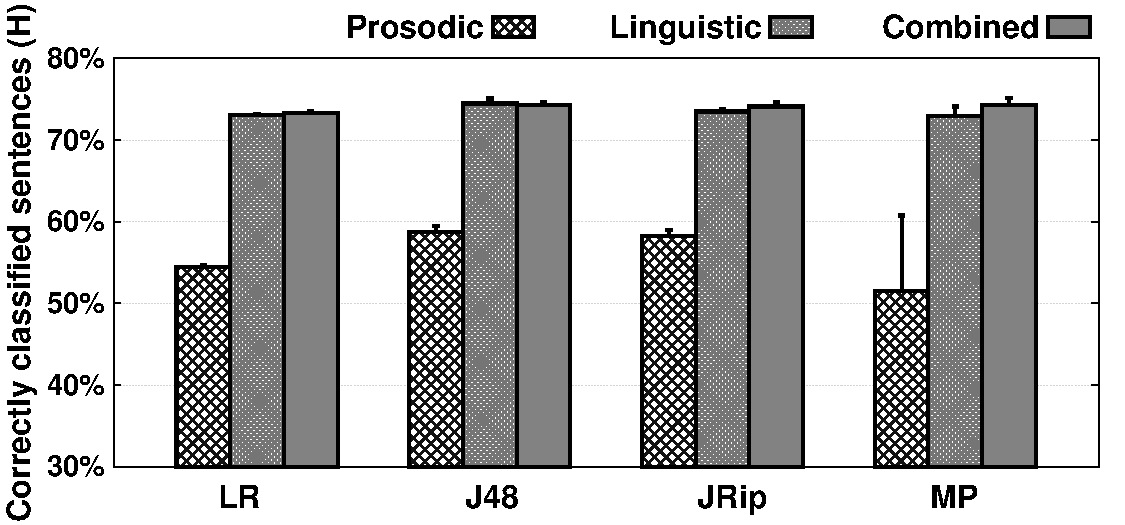
\includegraphics[scale=0.4]{Image/results/average_PLC_onManual_4colors_withSD_Gray.pdf}

\smallskip
{\footnotesize Analysis of the average classifier's performance when applied on \\\textbf{\color{purple}manual transcriptions}}
\end{center}

\smallskip
{\scriptsize
{\color{purple}$\Rightarrow$} the linguistic classifiers outperform the prosodic classifiers \\
{\vskip1ex\color{purple}$\Rightarrow$} the combination of linguistic and prosodic features does not provide any significant improvement on manual transcripts
}

\end{frame}


%==============================================================================================================
\begin{frame}[t]{Results on automatic transcriptions}

\begin{center}

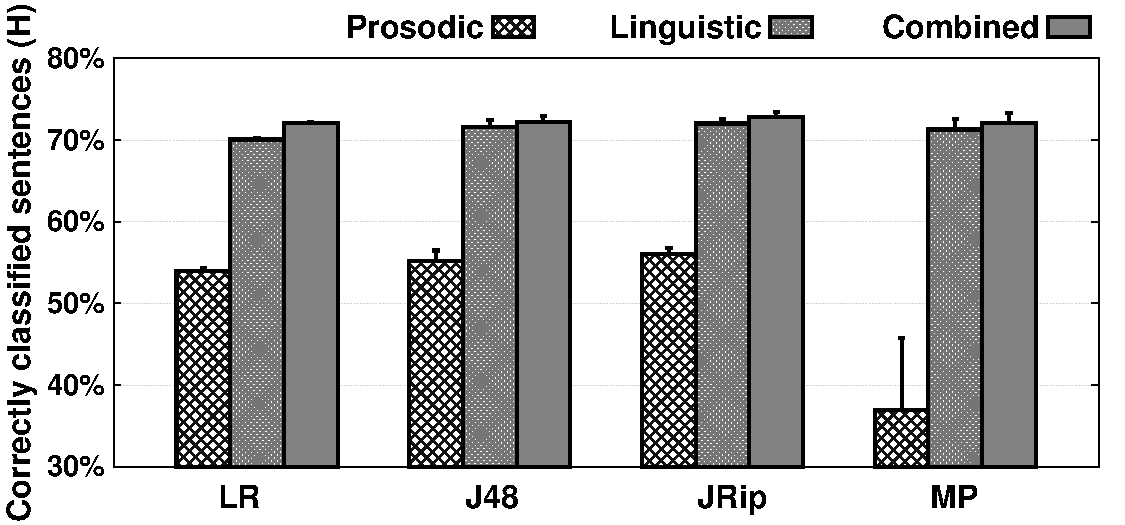
\includegraphics[scale=0.40]{Image/results/average_PLC_onAutomatic_4colors_withSD_Gray.pdf}

\smallskip
{\footnotesize Analysis of the average classifier's performance when applied on \\\textbf{\color{purple}automatic transcriptions}}
\end{center}


\smallskip
{\scriptsize
{\color{purple}$\Rightarrow$} the linguistic classifiers outperform the prosodic classifiers \\
{\vskip1ex\color{purple}$\Rightarrow$} ~3\% performance loss between the manual and the automatic transcriptions\\
{\vskip1ex\color{purple}$\Rightarrow$} the combination of linguistic and prosodic features provides a slight improvement on automatic transcription
}

\end{frame}


%==============================================================================================================
\begin{frame}[t]{Best results on manual and automatic transcriptions}

\bigskip


\begin{itemize}
\item {\scriptsize Confusion matrix between questions and statements obtained on \textbf{\color{purple}manual transcriptions (MLP, H=75.05\%)}}
\end{itemize}

\vskip-2ex
\begin{table}
\centering
\scriptsize
\begin{tabular}{p{1.7cm}|p{1cm}|p{1.6cm}|p{1.6cm}|p{2cm}}
\cline{2-4}
& number & classified as question & classified as statement &   \\ 
\end{tabular}

\begin{tabular}{|p{1.7cm}|p{1cm}|p{1.6cm}|p{1.6cm}|p{2cm}}
\cline{1-4}
question   &  831 & \textbf{603} & 228    & \textbf{ccQuestions=72.56\%} \\ \cline{1-4}
statement  & 7005 & 1559 & \textbf{5446}  & \textbf{ccStatements=77.74\%} \\ \cline{1-4}
\end{tabular}
\end{table}



\bigskip
\begin{itemize}
\item {\scriptsize Confusion matrix between questions and statements obtained on \textbf{\color{purple}automatic transcriptions (MLP, H=73.50\%)}}
\end{itemize}

\vskip-2ex
\begin{table}
\centering
\scriptsize
\begin{tabular}{p{1.7cm}|p{1cm}|p{1.6cm}|p{1.6cm}|p{2cm}}
\cline{2-4}
& number & classified as question & classified as statement &   \\ 
\end{tabular}

\begin{tabular}{|p{1.7cm}|p{1cm}|p{1.6cm}|p{1.6cm}|p{2cm}}
\cline{1-4}
question   &  831 & \textbf{611}  & 220   & \textbf{ccQuestions=73.60\%} \\ \cline{1-4}
statement  & 7005 & 1863 & \textbf{5142}  & \textbf{ccStatements=73.41\%} \\ \cline{1-4}
\end{tabular}
\end{table}


\end{frame}


%==============================================================================================================
\begin{frame}{Impact of different feature combinations}

\bigskip

\begin{center}

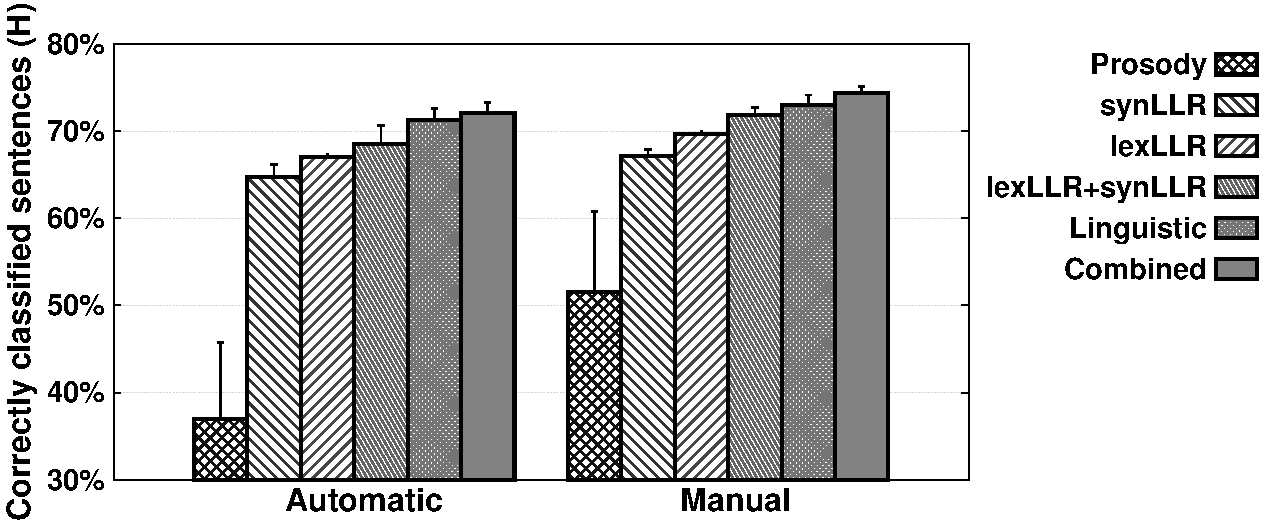
\includegraphics[scale=0.40]{Image/results/MP_averageStats_compareFeatures_withSD_Gray.pdf}

\smallskip
{\footnotesize Analysis of the average performance obtained with the MLP classifier when using \textbf{\color{purple}different feature combinations} on automatic and manual transcriptions}
\end{center}


\bigskip
{\scriptsize
{\color{purple}$\Rightarrow$} the most important linguistic feature is the lexical log-likelihood ratio (lexLLR) \\
{\vskip1ex\color{purple}$\Rightarrow$} the best results are obtained when combining all features
}


\end{frame}



%==============================================================================================================
\begin{frame}[t]{Impact of sentence boundaries}

\vskip0.8cm
{\footnotesize Assess the performance loss when the \textbf{\color{purple}sentence boundaries} are not perfect}

{\footnotesize 
\vskip4ex \hskip2ex $\rightarrow$ change the predefined sentence boundaries \\

	\vskip2ex\hskip9ex $\ast$ by shifting each boundary (left and right) with a random value of \\\hskip15ex {\scriptsize \{-300, -200, -100, +100, +200, +300\}ms }\\
	\vskip2ex\hskip9ex $\ast$ by shifting each boundary (left and right) with a random value of \\\hskip15ex {\scriptsize \{-1000, -800, -600, -400, -200, +200, +400, +600, +800, +1000\}ms} \\
	\vskip2ex\hskip9ex $\ast$ by finding the longest silence-enclosed sentence}

\end{frame}


%==============================================================================================================
\begin{frame}{Impact of sentence boundaries}

\vskip2ex

\only<1>
{
\textbf{Reference sentence:}

	\vskip1ex\hskip5ex "que fallait -il faire" [947090,948370]
	
{\scriptsize	
\begin{table}[h]
\centering
\begin{tabular}{|r|r|r|r|}
\hline
{\color{gray}946230}  & {\color{gray}946290} & {\color{gray}++micro++}   	& {\color{gray} 60 [ms]}	\\
{\color{gray}946300}  & {\color{gray}946350} & {\color{gray}à}			& {\color{gray} 50 [ms]}	\\
{\color{gray}946360}  & {\color{gray}946660} & {\color{gray}travers}		& {\color{gray}300 [ms]}	\\
{\color{gray}946670}  & {\color{gray}946760} & {\color{gray}le}			& {\color{gray} 90 [ms]}	\\
{\color{gray}946770}  & {\color{gray}947020} & {\color{gray}monde}		& {\color{gray}250 [ms]}	\\ \hline
\textbf{947030}       & {\color{gray}947160} & \textbf{$\textless$sil$\textgreater$}  	& {\color{gray}130 [ms]}	\\ 
{\color{gray}947230}  & {\color{gray}947450} & \textbf{++resp++} 		& {\color{gray}220 [ms]}	\\ 
{\color{gray}947460}  & {\color{gray}947650} & \textbf{que}			& {\color{gray}190 [ms]}	\\
{\color{gray}947660}  & {\color{gray}947920} & \textbf{fallait} 		& {\color{gray}260 [ms]}	\\
{\color{gray}947930}  & {\color{gray}948080} & \textbf{-il}			& {\color{gray}150 [ms]}	\\
{\color{gray}948090}  & \textbf{948350} & \textbf{faire}  			& {\color{gray}260 [ms]}	\\ \hline
{\color{gray}948360}  & {\color{gray}948390} & {\color{gray}eh}			& {\color{gray} 30 [ms]}	\\
{\color{gray}948400}  & {\color{gray}948530} & {\color{gray}bien} 		& {\color{gray}130 [ms]}	\\
{\color{gray}948540}  & {\color{gray}948670} & {\color{gray}il} 		& {\color{gray}130 [ms]}	\\
{\color{gray}948680}  & {\color{gray}948870} & {\color{gray}fallait} 		& {\color{gray}190 [ms]}	\\
{\color{gray}948880}  & {\color{gray}949310} & {\color{gray}choisir} 		& {\color{gray}430 [ms]}	\\ 
{\color{gray}949320}  & {\color{gray}949400} & {\color{gray}++rire++} 		& {\color{gray} 80 [ms]}	\\ \hline
\end{tabular}
\end{table}
}
}

\only<2>
{
\textbf{Modified borders {\color{purple}$\pm$ 300ms}: } [+200,+300ms]

	\vskip1ex\hskip5ex "que fallait -il faire eh bien il" [947290,948670]
	
{\scriptsize	
\begin{table}[h]
\centering
\begin{tabular}{|r|r|r|r|}
\hline
{\color{gray}946230}  	& {\color{gray}946290} 	& {\color{gray}++micro++}   			& {\color{gray} 60 [ms]}	\\
{\color{gray}946300}  	& {\color{gray}946350} 	& {\color{gray}à}				& {\color{gray} 50 [ms]}	\\
{\color{gray}946360}  	& {\color{gray}946660} 	& {\color{gray}travers}				& {\color{gray}300 [ms]}	\\
{\color{gray}946670}  	& {\color{gray}946760} 	& {\color{gray}le}				& {\color{gray} 90 [ms]}	\\
{\color{gray}946770}  	& {\color{gray}947020} 	& {\color{gray}monde}				& {\color{gray}250 [ms]}	\\	
{\color{gray}947030} 	& {\color{gray}947160} 	& {\color{gray}$\textless$sil$\textgreater$}  	& {\color{gray}130 [ms]}	\\ \hline
\textbf{947230} 	& {\color{gray}947450} 	& \textbf{++resp++}				& {\color{gray}220 [ms]}	\\ 
{\color{gray}947460}	& {\color{gray}947650} 	& \textbf{que}					& {\color{gray}190 [ms]}	\\
{\color{gray}947660}	& {\color{gray}947920} 	& \textbf{fallait} 				& {\color{gray}260 [ms]}	\\
{\color{gray}947930}  	& {\color{gray}948080} 	& \textbf{-il}					& {\color{gray}150 [ms]}	\\
{\color{gray}948090}	& {\color{gray}948350} 	& \textbf{faire}  				& {\color{gray}260 [ms]}	\\ 
{\color{gray}948360}  	& {\color{gray}948390} 	& \textbf{\color{blue}eh}			& {\color{gray} 30 [ms]}	\\
{\color{gray}948400}  	& {\color{gray}948530} 	& \textbf{\color{blue}bien}			& {\color{gray}130 [ms]}	\\
{\color{gray}948540}  	& \textbf{948670} 	& \textbf{\color{blue}il} 			& {\color{gray}130 [ms]}	\\ \hline
{\color{gray}948680}	& {\color{gray}948870} 	& {\color{gray}fallait} 			& {\color{gray}190 [ms]}	\\
{\color{gray}948880}  	& {\color{gray}949310} 	& {\color{gray}choisir} 			& {\color{gray}430 [ms]}	\\ 
{\color{gray}949320}  	& {\color{gray}949400} 	& {\color{gray}++rire++} 			& {\color{gray} 80 [ms]}	\\ \hline
\end{tabular}
\end{table}
}
}


\only<3>
{
\textbf{Modified borders {\color{purple}$\pm$ 1000ms}: } [-400ms,-600ms]

	\vskip1ex\hskip5ex "le monde que fallait" [946690,947770]
{\scriptsize	
\begin{table}[h]
\centering
\begin{tabular}{|r|r|r|r|}
\hline
{\color{gray}946230}  	& {\color{gray}946290} 	& {\color{gray}++micro++}    	& {\color{gray} 60 [ms]}	\\
{\color{gray}946300}  	& {\color{gray}946350} 	& {\color{gray}à}		& {\color{gray} 50 [ms]}	\\
{\color{gray}946360}  	& {\color{gray}946660} 	& {\color{gray}travers}		& {\color{gray}300 [ms]}	\\ \hline
\textbf{946670}  	& {\color{gray}946760} 	& \textbf{\color{blue}le}	& {\color{gray} 90 [ms]}	\\
{\color{gray}946770}  	& {\color{gray}947020} 	& \textbf{\color{blue}monde}	& {\color{gray}250 [ms]}	\\	
{\color{gray}947030} 	& {\color{gray}947160} 	& \textbf{$\textless$sil$\textgreater$} 	& {\color{gray}130 [ms]}	\\ 
{\color{gray}947230}  	& {\color{gray}947450} 	& \textbf{++resp++} 			& {\color{gray}220 [ms]}	\\ 
{\color{gray}947460}	& {\color{gray}947650} 	& \textbf{que}			& {\color{gray}190 [ms]}	\\
{\color{gray}947660}	& \textbf{947920} 	& \textbf{fallait} 		& {\color{gray}260 [ms]}	\\ \hline
{\color{gray}947930}  	& {\color{gray}948080} 	& {\color{gray}-il}		& {\color{gray}150 [ms]}	\\
{\color{gray}948090}	& {\color{gray}948350} 	& {\color{gray}faire}  		& {\color{gray}260 [ms]}	\\ 
{\color{gray}948360}  	& {\color{gray}948390} 	& {\color{gray}eh}		& {\color{gray} 30 [ms]}	\\
{\color{gray}948400}  	& {\color{gray}948530} 	& {\color{gray}bien}		& {\color{gray}130 [ms]}	\\
{\color{gray}948540}  	& {\color{gray}948670} 	& {\color{gray}il}		& {\color{gray}130 [ms]}	\\ 
{\color{gray}948680}	& {\color{gray}948870} 	& {\color{gray}fallait} 	& {\color{gray}190 [ms]}	\\
{\color{gray}948880}  	& {\color{gray}949310} 	& {\color{gray}choisir} 	& {\color{gray}430 [ms]}	\\ 
{\color{gray}949320}  	& {\color{gray}949400} 	& {\color{gray}++rire++} 	& {\color{gray} 80 [ms]}	\\ \hline
\end{tabular}
\end{table}
}
}


\only<4>
{
\textbf{Modified borders:} {\small the longest {\color{purple}silence-enclosed} sentence}

	\vskip1ex\hskip5ex "que fallait -il faire eh bien il fallait choisir" [947460,949310]
	
{\scriptsize	
\begin{table}[h]
\centering
\begin{tabular}{|r|r|r|r|}
\hline
{\color{gray}946230}  	& {\color{gray}946290} 	& {\color{gray}++micro++}    			& {\color{gray} 60 [ms]}\\
{\color{gray}946300}  	& {\color{gray}946350} 	& {\color{gray}à}				& {\color{gray} 50 [ms]}\\
{\color{gray}946360}  	& {\color{gray}946660} 	& {\color{gray}travers}				& {\color{gray}300 [ms]}\\
{\color{gray}946670}  	& {\color{gray}946760} 	& {\color{gray}le}				& {\color{gray} 90 [ms]}\\
{\color{gray}946770}  	& {\color{gray}947020} 	& {\color{gray}monde}				& {\color{gray}250 [ms]}\\ 
{\color{gray}947030}  	& {\color{gray}947160} 	& {\color{gray}$\textless$sil$\textgreater$}  	& {\color{gray}130 [ms]}\\ 
{\color{gray}947230} 	& {\color{gray}947450} 	& {\color{gray}++resp++} 			& {\color{gray}220 [ms]}\\ \hline
\textbf{947460}		& {\color{gray}947650} 	& \textbf{que}					& {\color{gray}190 [ms]}\\
{\color{gray}947660}	& {\color{gray}947920} 	& \textbf{fallait} 				& {\color{gray}260 [ms]}\\
{\color{gray}947930}  	& {\color{gray}948080} 	& \textbf{-il}					& {\color{gray}150 [ms]}\\
{\color{gray}948090}	& {\color{gray}948350} 	& \textbf{faire}  				& {\color{gray}260 [ms]}\\ 
{\color{gray}948360}  	& {\color{gray}948390} 	& \textbf{\color{blue}eh}			& {\color{gray} 30 [ms]}\\
{\color{gray}948400}  	& {\color{gray}948530} 	& \textbf{\color{blue}bien} 			& {\color{gray}130 [ms]}\\
{\color{gray}948540}  	& {\color{gray}948670} 	& \textbf{\color{blue}il} 			& {\color{gray}130 [ms]}\\
{\color{gray}948680}	& {\color{gray}948870} 	& \textbf{\color{blue}fallait} 			& {\color{gray}190 [ms]}\\
{\color{gray}948880} 	& \textbf{949310} 	& \textbf{\color{blue}choisir} 			& {\color{gray}430 [ms]}\\ \hline
{\color{gray}949320}  	& {\color{gray}949400} 	& {\color{gray}++rire++} 			& {\color{gray} 80 [ms]}\\ \hline
\end{tabular}
\end{table}
}
}


\end{frame}



%==============================================================================================================
\begin{frame}[t]{Impact of sentence boundaries}

\vskip0.1cm

\smallskip
\begin{center}
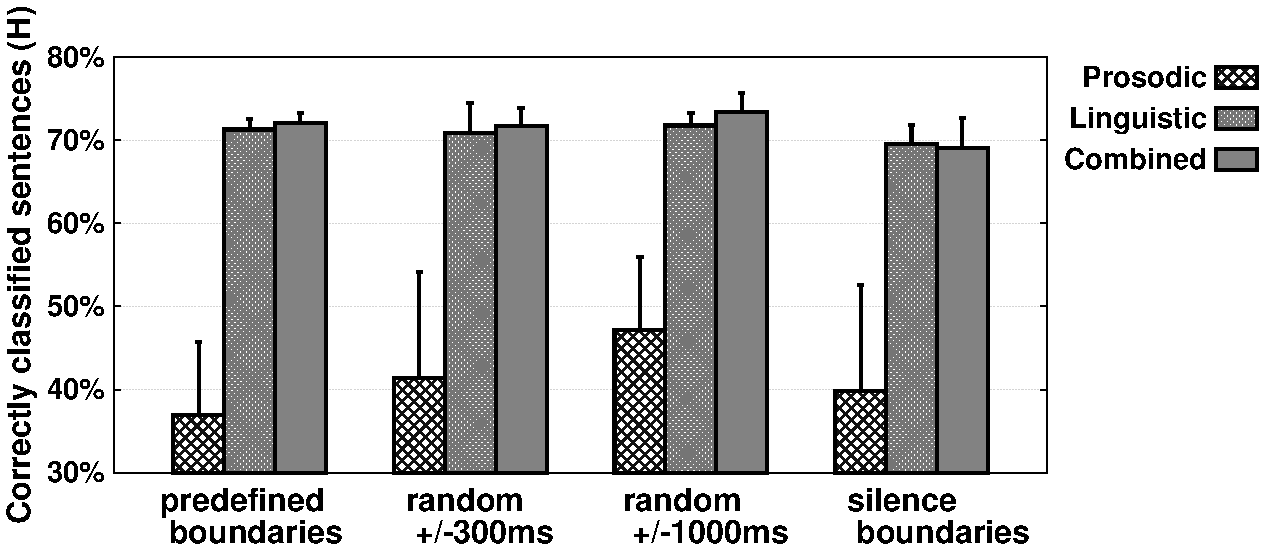
\includegraphics[scale=0.38]{Image/results/MP_averageStats_differentBorders_Gray.pdf}
\smallskip

{\footnotesize Analysis of the average performance obtained with the MLP classifier on automatic transcriptions when modifying the predefined boundaries}
\end{center}

\smallskip
{\scriptsize
{\color{purple}$\Rightarrow$} even if an automatic segmentation module wrongly assigns the sentence boundaries, our classifier still manages to correctly classify
the question/statements entries between 69\% and 72\%
}

\end{frame}



%==============================================================================================================
\section{Conclusions and future work}
\begin{frame}[t]{Conclusions and future work}
\setcounter{framenumber}{19}

\vskip0.3cm

\begin{itemize}
\item Conclusions 
	\vskip0.1cm
	\begin{itemize}
	\item the prosodic classifier gives poor classification results
	\vskip2ex
	\item the linguistic classifier provides by far better results \\(72\% on ASR transcripts, 74\% on manual transcripts)
	\vskip2ex
	\item the combination of prosodic and linguistic features provides a slight improvement when applied on automatic transcriptions
	\vskip2ex
	\item all 13 features are useful in detecting questions and statements
	\vskip2ex
	\item even if an automatic segmentation module wrongly assigns the sentence boundaries, our classifier still manages to correctly classify the question/statements
entries between 69\% and 72\%
	\end{itemize}

\vskip0.3cm
\item Investigate further 
	\vskip0.1cm
	\begin{itemize}
	\item the use of confidence measures inside the classifier
	\end{itemize}
\end{itemize}


\end{frame}


%==============================================================================================================
\begin{frame}[plain]

\begin{center}
\textcolor{polyured}{\huge \textbf{Thank you \\\vskip0.2cm for your attention !}}
\end{center}

\end{frame} 



%\setbeamertemplate{footline}[page number]{}
%\setbeamertemplate{footline}{}
%==============================================================================================================
%\begin{frame}{Annexe}
%\end{frame}

\end{document}


